% !TeX program=pdflatex
\documentclass{article}
\usepackage[utf8]{inputenc}
\usepackage{MyChem}
\usepackage{MyStandard}
\usepackage{courier}
\usepackage{booktabs}
\usepackage{graphicx}
%%\usepackage{tabto}
%% \usepackage{tabu}
\usepackage{longtable}
\usepackage{enumerate}
\usepackage[symbol]{footmisc}
\usepackage{gensymb} % enables degree sign
\usepackage{tabularx}
\usepackage{multirow}

\newcommand\eint{\enmat{E^{\te{int}}}}
\newcommand\ecc{\enmat{\eint_{\te {CC}}}}
\newcommand\kmo{\enmat{\te {kJ/mol}}}

\begin{document}


\section*{H$_2$O+H }
\large$\ecc=-0.40\ \kmo$ \\
%\ph{ah}
%\vskip-2cm
%\large\textbf{H$_2$O+H} \\

\raisebox{.4cm}{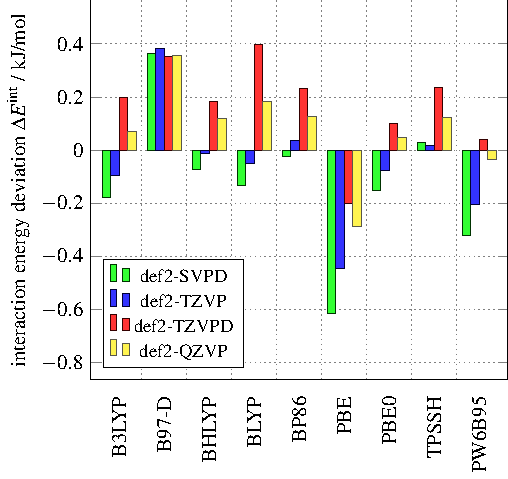
\includegraphics[width=.48\textwidth]{H2O+H+NoD3.pdf}}
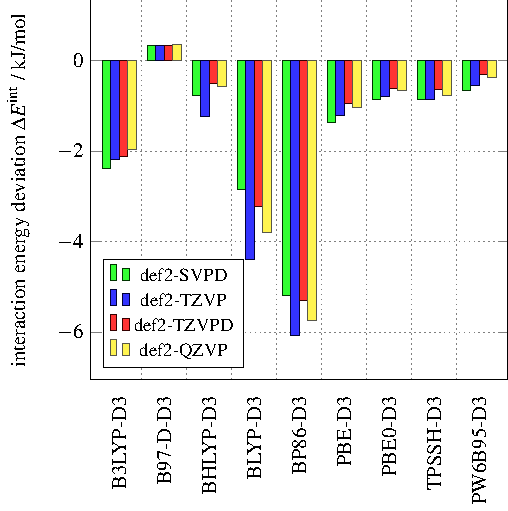
\includegraphics[width=.48\textwidth]{H2O+H+D3.pdf}

\section*{H$_2$O+H$_2$O}
\large$\ecc=-20.80\ \kmo$ \\
%\large\textbf{H$_2$O+H$_2$O} \\
{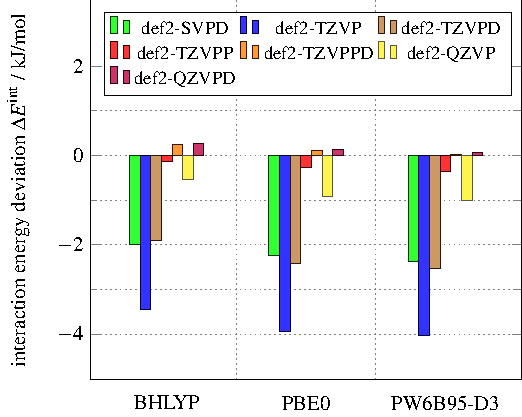
\includegraphics[width=.48\textwidth]{H2O+H2O+BasisCompare.pdf}}
\raisebox{-1cm}{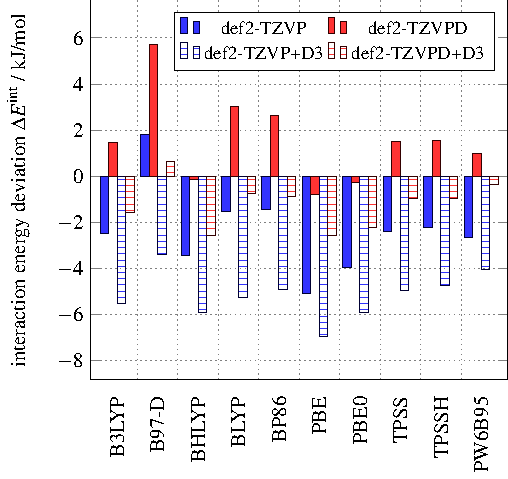
\includegraphics[width=.48\textwidth]{H2O+H2O+TZVPCompare.pdf}}

\section*{H$_2$O+O}
\large$\ecc=-6.72\ \kmo$ \\
%\large\textbf{H$_2$O+O} \\
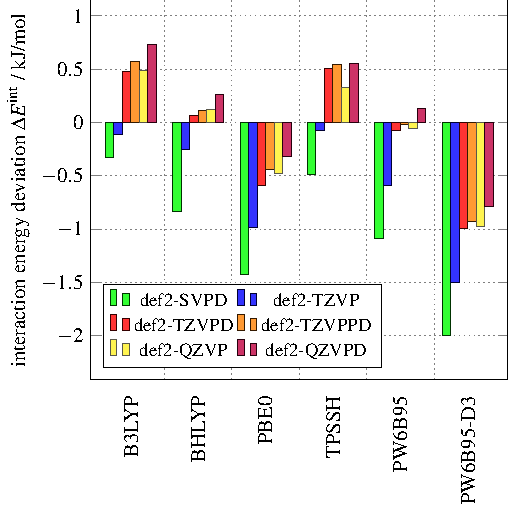
\includegraphics[width=.48\textwidth]{H2O+O+FuncCompare.pdf}
%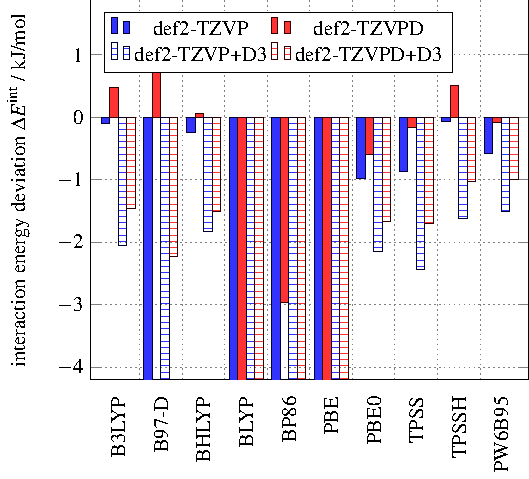
\includegraphics[width=.48\textwidth]{H2O+O+TZVPCompare.pdf}
%
%\begin{figure}[h]
%\centering
%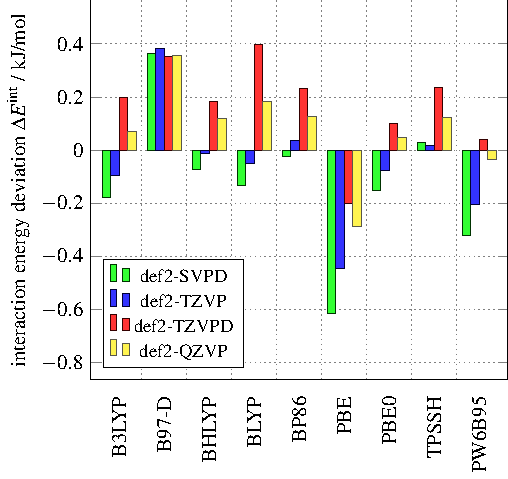
\includegraphics[width=.48\textwidth]{H2O+H+NoD3.pdf}
%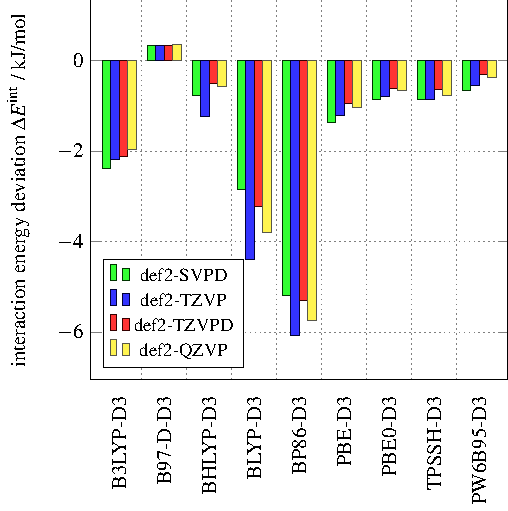
\includegraphics[width=.48\textwidth]{H2O+H+D3.pdf}
%\end{figure}
%
%%\section*{H$_2$O+H$_2$O}
%\begin{figure}[h]
%\centering
%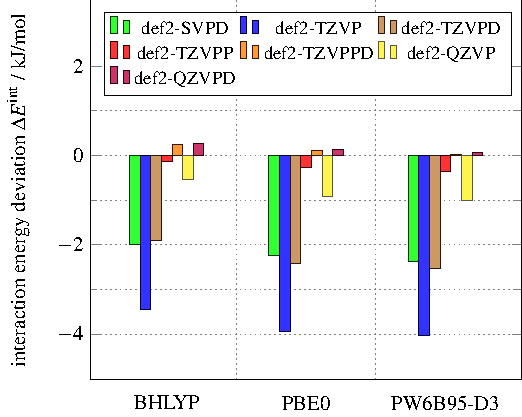
\includegraphics[width=.48\textwidth]{H2O+H2O+BasisCompare.pdf}
%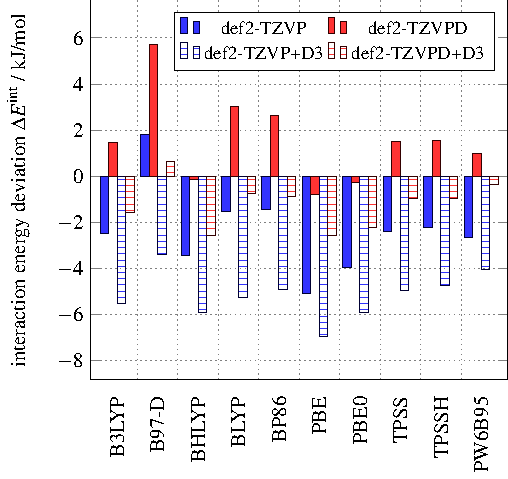
\includegraphics[width=.48\textwidth]{H2O+H2O+TZVPCompare.pdf}
%\end{figure}
%
%%\section*{H$_2$O+O}
%\begin{figure}[h]
%\centering
%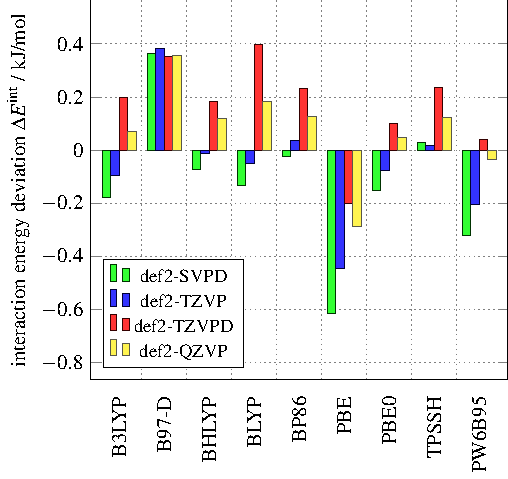
\includegraphics[width=.48\textwidth]{H2O+H+NoD3.pdf}
%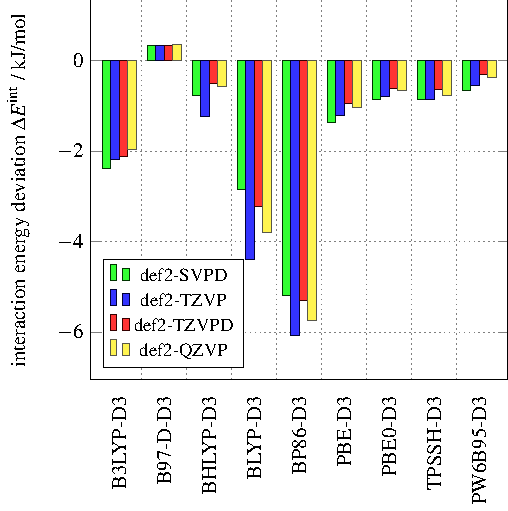
\includegraphics[width=.48\textwidth]{H2O+H+D3.pdf}
%\end{figure}


\end{document}